% !TEX root = Master.tex

The source literature for this section can be found in the first chapter of \cite{nagarajan2013bayesian}, where elements of graph theory are introduced.
\\

A graph $G=(\mathbf{V}, A)$ consist of a non-empty set of \textit{nodes} or \textit{vertices} $\bm{V}$ and a finite set $A$ of pairs of vertices calles \textit{arcs}, \textit{links}, or \textit{edges}. Each arc $a=(u, v)$ comprises of as an ordered or unordered pair of nodes, which are \textit{connected by} and \textit{incident} on the arc $a$ or \textit{adjacent} to each other an therefore $u$ and $v$ can also be called \textit{neighbors}. \\

For the purpose of this thesis, we limit the theory to ordered node pairs. If $(u,v)$ is an ordered pair, then $u$ is said to be the \textit{tail} of the arc $a$ and $v$ the head of $a$, i.e. $a$ is called \textit{directed} from $u$ to $v$. The usual representation is $(u \rightarrow v)$. It is also said that arc $a$ \textit{leaves} or is \textit{outgoing} for $u$ and that it \textit{enters} or is \textit{incoming} for $v$. If a graph $G$ consist of directed arcs only and has no cycles\footnote{i.e. No node can be traversed back to itself.}, it is called a \textit{\ac{DAG}}. \\ In the example of \autoref{fig:dag_example}, the node set is $\mathbf{V}=\{\mathrm{A}, \mathrm{B}, \mathrm{C}, \mathrm{D}, \mathrm{E}\}$ and the graph is characterized by the arc set $A=\{(A \rightarrow B),(C \rightarrow A),(D \rightarrow B),(C \rightarrow D),(C \rightarrow E)\}$. As arcs are directed, $C \rightarrow D$ and $D \rightarrow C$ are different and due to acyclicity it is impossible for both arcs to be in the graph because there can be at most one arc between each pair of nodes. Hence, $C \rightarrow D \in A$ while $D \rightarrow E \notin A$.
\\

A sequence of arcs connecting two nodes (\textit{end-nodes}) is called a \textit{path} and is denoted with the sequence of nodes $\left(v_{1}, v_{2}, \ldots, v_{n}\right)$ incident on those arcs. A path between two end-nodes is assumed to be unique. If node $v_i$ precedes node $v_j$, there can be no arc from $v_j$ to $v_i$. In this case, $v_i$ is called an \textit{ancestor} of $v_j$ and $v_j$ is called a \textit{descendant} of $v_i$. If these two nodes are adjacent, $v_i$ is called a parent of $v_j$ and $v_j$ is called a child of $v_i$.
\\

\begin{figure}[H]
\centering
  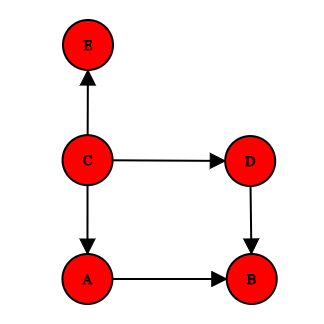
\includegraphics[width=0.45\linewidth]{figures/dag_example.png}
  \caption{Example of a directed acyclic graph}
  \label{fig:dag_example}
\end{figure}





